\documentclass[answers,12pt,addpoints]{exam}
\usepackage{graphicx,multicol}
\usepackage{charter,amsmath,amssymb}
\usepackage{eulervm}
\usepackage[letterpaper,margin=1in]{geometry}
\pagestyle{headandfoot}
\runningheadrule
\runningheader{\bf Math 265}
{\bf Exam One, Page \thepage\ of \numpages}
{\bf 6 February 2015}
\firstpagefooter{}{}{}
\runningfooter{}{}{}
\let\cos\relax\DeclareMathOperator{\cos}{\mathsf{cos}}
\let\sin\relax\DeclareMathOperator{\sin}{\mathsf{sin}}
\let\ln\relax\DeclareMathOperator{\ln}{\mathsf{ln}}
\let\lim\relax\DeclareMathOperator*{\lim}{\mathsf{lim}}
\everymath{\displaystyle}
\begin{document}
\begin{center}
\huge Math 265 Exam One\\
\LARGE Spring 2015
\end{center}

\ifprintanswers\else
\begin{center}
\fbox{\fbox{\parbox{5.5in}{
This exam has \numquestions~questions.
It has been printed on \numpages~pages and is worth \numpoints~points.
Answer all the questions in the spaces provided.
%The last page has been left blank for your calculations.
Although you may use any calculator on this exam,
you must clearly indicate how you arrived at your answers
in order to receive maximum credit.
By signing below, you pledge that you
\begin{enumerate}
\item will not communicate to any person in any conceivable way anything
about the contents of this exam
until all students have taken it, and
\item have not been the recipient of such communication from anyone else.
\end{enumerate}}}}
\end{center}
\vspace{.2in}
\makebox[\textwidth]{Your signature:\enspace\hrulefill}\\
\vspace{.2in}\\
\makebox[\textwidth]{Your name:\enspace\hrulefill}\\
\begin{center}\gradetable[h][questions]\end{center}
\fi

\begin{questions}
\begin{multicols}{2}
\question[10] Find and classify all
the critical points of \[f\left(x,y\right)
=x^3+y^3-3x-3y\] as local maxima, local minima,
saddle points, or none of these.
The contour plot of $f$ is shown at the right.
\begin{center}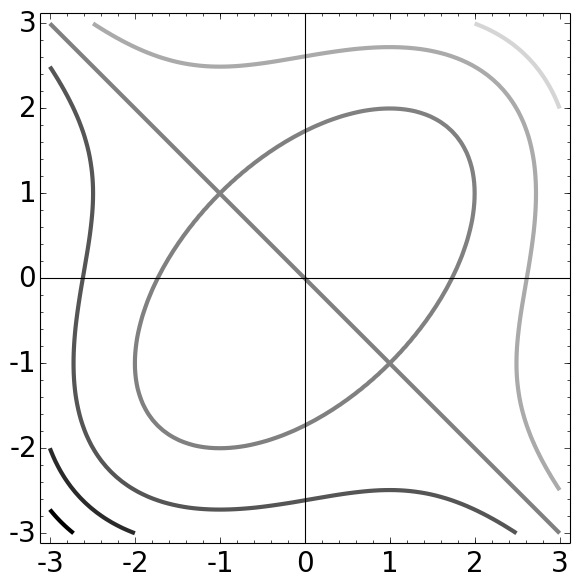
\includegraphics[scale=.4]{Saddles}\end{center}
\end{multicols}

\end{questions}
\end{document}
